% Graphical abstract concept 2: prediction meets measurement.
% Left: the asynchronous run yields a timing record; the barrierized twin is the
% same sampler with a barrier drawn in. Right: the stripped predictor scatter
% (python: ../py/ga2_predictor_panel.py -> ../out/ga2_predictor_panel.pdf).
\documentclass[tikz,border=4pt]{standalone}
\usepackage{newtxtext,newtxmath}
\usepackage{graphicx}
\usetikzlibrary{arrows.meta,positioning,calc,patterns}
\definecolor{async}{HTML}{0072B2}
\definecolor{sync}{HTML}{D55E00}

\begin{document}
\begin{tikzpicture}[font=\small,>=Stealth,x=1cm,y=1cm]
\pgfmathsetmacro{\laneh}{0.22}
\pgfmathsetmacro{\lanegap}{0.08}
\pgfmathsetmacro{\xs}{0.85}   % time unit in cm for the lane cartoons
\pgfmathsetmacro{\win}{4.4}   % cartoon window, time units
\def\durations{{{0.9,0.5,1.1,0.6},{0.4,1.6,0.5,0.8},{1.3,0.6,0.7,1.0},{0.6,0.8,1.5,0.5}}}
\def\genmax{{1.3,1.6,1.5}}    % slowest simulation of generations 1-3

\node[font=\bfseries,anchor=west] at (0,3.9) {The barrier's cost is predicted from the asynchronous run alone};

%% asynchronous run (top left)
\begin{scope}[shift={(0,3.0)}]
\node[anchor=south west,font=\footnotesize\bfseries,text=async] at (0,0.08) {Asynchronous run};
\foreach \w in {1,...,4} {
  \pgfmathsetmacro{\yb}{-(\w-1)*(\laneh+\lanegap)}
  \xdef\tcur{0}
  \foreach \j in {0,...,7} {
    \pgfmathsetmacro{\col}{int(mod(\j,4))}
    \pgfmathsetmacro{\d}{\durations[\w-1][\col]}
    \pgfmathsetmacro{\ts}{\tcur}
    \pgfmathsetmacro{\te}{\ts+\d}
    \ifdim \ts pt<\win pt
      \pgfmathsetmacro{\tclip}{min(\te,\win)}
      \fill[async!85,draw=white,line width=0.4pt] (\ts*\xs,\yb) rectangle (\tclip*\xs,\yb+\laneh);
    \fi
    \xdef\tcur{\te}
  }
}
\node[anchor=north west,font=\scriptsize,align=left,text width=4.3cm] at (0,-1.3)
  {record every simulation's duration $D_i$ and the rate $T_{\text{async}}$;
   predict $T_{\text{sync}} = W/\mathbb{E}[\max_{i\le W} D_i]$ by resampling the $D_i$};
\end{scope}

%% barrierized twin (bottom left)
\begin{scope}[shift={(0,-0.3)}]
\node[anchor=south west,font=\footnotesize\bfseries,text=sync] at (0,0.08) {Barrierized twin: same sampler + barrier};
\xdef\Bprev{0}
\foreach \g in {1,...,3} {
  \pgfmathsetmacro{\gmax}{\genmax[\g-1]}
  \pgfmathsetmacro{\Bnext}{\Bprev+\gmax}
  \foreach \w in {1,...,4} {
    \pgfmathsetmacro{\yb}{-(\w-1)*(\laneh+\lanegap)}
    \pgfmathsetmacro{\d}{\durations[\w-1][\g-1]}
    \pgfmathsetmacro{\te}{\Bprev+\d}
    \fill[sync!85,draw=white,line width=0.4pt] (\Bprev*\xs,\yb) rectangle (\te*\xs,\yb+\laneh);
    \ifdim \te pt<\Bnext pt
      \fill[pattern=north east lines,pattern color=black!50] (\te*\xs,\yb) rectangle (\Bnext*\xs,\yb+\laneh);
    \fi
  }
  \draw[sync,dashed,line width=0.7pt] (\Bnext*\xs,0.05) -- (\Bnext*\xs,{-4*(\laneh+\lanegap)+\lanegap-0.05});
  \xdef\Bprev{\Bnext}
}
\node[anchor=north west,font=\scriptsize,align=left,text width=4.3cm] at (0,-1.3)
  {measure its rate $T_{\text{sync}}$ directly; nothing else in the sampler changes};
\end{scope}

%% arrows into the scatter
\draw[->,async,thick] (4.5,2.4) -- (5.5,2.4) node[midway,above,font=\scriptsize,text=async] {predicted};
\draw[->,sync,thick] (4.5,-0.9) -- (5.5,-0.9) node[midway,above,font=\scriptsize,text=sync] {measured};

%% scatter
\node[anchor=west,inner sep=0pt] at (5.6,0.9) {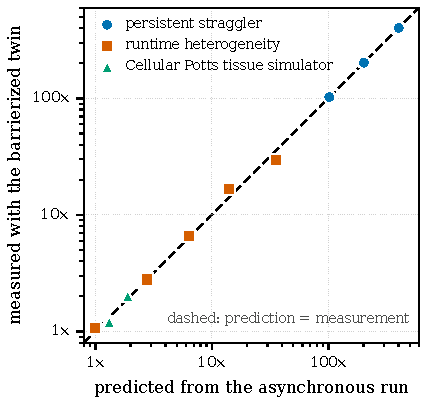
\includegraphics[height=5.6cm]{../out/ga2_predictor_panel.pdf}};

\node[anchor=north west,font=\scriptsize,align=left,text width=12.4cm] at (0,-2.5)
  {Predicted against measured barrier cost, $1.2\times$ to $400\times$: within $1\%$ under a persistent straggler,
   $20\%$ under lognormal runtime heterogeneity, $10\%$ on a Cellular Potts tissue simulator.};
\end{tikzpicture}
\end{document}
